\bookchapter{第六十章：搭建開發環境——Xcode 與第一個專案}

\chapterintro{工欲善其事，必先利其器。這一章咱們把“廚房”搭好：裝好 Xcode、跑通模擬器、建立人生第一個 iOS 專案，再把工程結構拆開看個明白。裝好環境之後，你會第一次看到自己寫的程式碼變成一個能點的按鈕——這個瞬間，很多人會記一輩子。}

\booksection{一、準備一臺 Mac}

先說門檻：iOS 開發必須在 macOS 上進行。如果你沒有 Mac，選項有三：買一臺（哪怕是二手 Mac mini 或 MacBook Air 都夠用）、短期租雲 Mac、或者先讀第八篇《安卓開發實戰篇》（Windows 就能幹）。

\begin{center}
\begin{tabularx}{\linewidth}{|X|X|X|}
\hline
\textbf{配置項} & \textbf{最低要求} & \textbf{舒適線（推薦）} \tabularnewline
\hline
晶片 & Apple Silicon（M1 起） & M2 及更新 \tabularnewline
記憶體 & 8GB & 16GB \tabularnewline
磁碟 & 預留 40GB+（Xcode 本體很胖） & 256GB 起步 \tabularnewline
系統 & 最新 macOS & 保持自動更新 \tabularnewline
\hline
\end{tabularx}
\end{center}

\begin{center}\small\color{gray}Mac 開發機配置參考（2026 年 8 月）\end{center}

\begin{tcbinfo}{小貼士：沒有 Mac 也能先學語言}
iPad 上免費的 Swift Playgrounds 能學 Swift 語言基礎（不用 Mac）；甚至 iPhone 上也能裝。先把第 61 章的語言知識在 Playgrounds 裡玩熟，等拿到 Mac 後直接起飛。磨刀不誤砍柴工，說的就是這個。

\end{tcbinfo}

\booksection{二、安裝 Xcode}

Xcode 是蘋果官方的整合開發環境，免費。三步裝好：

\begin{enumerate}
  \item Mac 上開啟 App Store，搜尋 "Xcode"，點安裝——注意它有好幾個 GB，找個網速好的時段；
  \item 裝完首次啟動，同意協議、裝完元件（自動完成）；
  \item 選單 Xcode Settings Locations，確認 Command Line Tools 已選中——命令列工具是很多指令碼和第三方工具的前提。
\end{enumerate}

\begin{tcbwarn}{注意：版本和系統的"匹配遊戲"}
新 Xcode 往往要求最新 macOS，舊 Mac 則會卡在老版本。上架 App Store 時，蘋果會要求用較新的 Xcode 構建（通常給一個寬限期）。所以系統更新別拖太久——iOS 開發者是“追新版”最勤快的一群人。

\end{tcbwarn}

\booksection{三、建立你的第一個專案}

開啟 Xcode Create New Project 選 iOS App 模板，然後填：

\begin{center}
\begin{tabularx}{\linewidth}{|X|X|X|}
\hline
\textbf{配置項} & \textbf{填什麼} & \textbf{說明} \tabularnewline
\hline
Product Name & MyFirstApp & 應用程式名稱字 \tabularnewline
Team & 你的 Apple ID（免費） & 簽名用，個人帳號即可 \tabularnewline
Organization Identifier & com.example & 和 Product Name 拼成包標識 \tabularnewline
Interface & SwiftUI & 本書主線框架 \tabularnewline
Language & Swift & 不解釋 \tabularnewline
\hline
\end{tabularx}
\end{center}

\begin{center}\small\color{gray}建立專案要填的五件事\end{center}

點 Create 後，Xcode 會生成一個能直接跑的專案。左上角選一臺模擬器（比如 iPhone 17），點 > 執行——幾秒後，模擬器螢幕上出現一個寫著 “Hello, world!” 的視窗。你的第一個 iOS App 已經誕生了。

\booksection{四、工程結構拆解：每個檔案是幹嘛的}

左側是工程導航器，新手只需認識這幾個：

\begin{center}
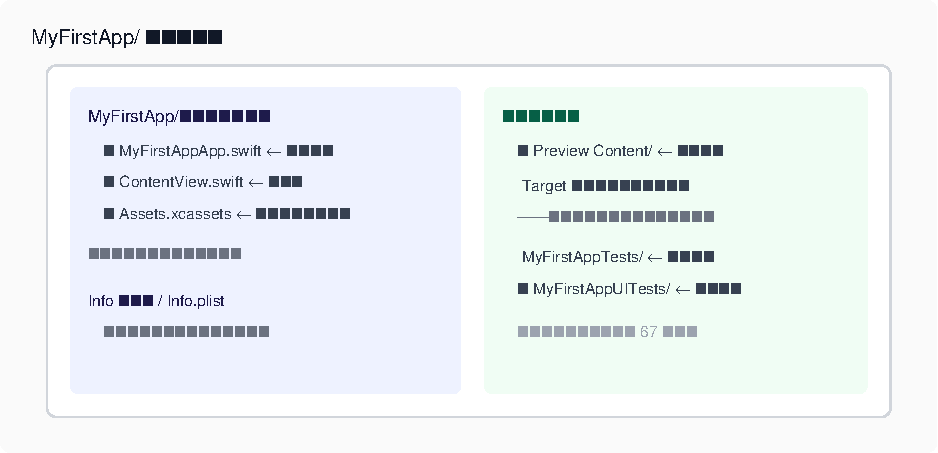
\includegraphics[width=0.92\linewidth]{figures/fig-di-liu-shi-zhang-1}
\\[2pt]\small 圖 2：新手必懂的 Xcode 工程結構
\end{center}

\begin{itemize}
  \item MyFirstAppApp.swift：程式入口，SwiftUI 裡它只有幾行——"啟動，然後顯示主介面"；
  \item ContentView.swift：主介面檢視，你現在看到的一切都在這裡；
  \item Assets.xcassets：資源倉庫——圖示、圖片、顏色都放這；
  \item Target 設定：點左側藍色工程圖示進去，版本號、最低 iOS 版本、簽名都在裡面。App 顯示名、圖示也在這配置。
\end{itemize}

\booksection{五、真機除錯：把 App 裝進你的 iPhone}

\booksection{五、Xcode 效率技巧：新手的五個“快速鍵外掛”}

用熟這幾個，你會顯得“很專業”：

\begin{center}
\begin{tabularx}{\linewidth}{|X|X|X|}
\hline
\textbf{操作} & \textbf{快速鍵} & \textbf{作用} \tabularnewline
\hline
執行 & CmdR & 編譯並跑起來 \tabularnewline
開啟/切換畫布預覽 & OptionCmd & 所見即所得的開關 \tabularnewline
格式化縮排 & CtrlI & 自動整理選中程式碼的縮排 \tabularnewline
快速開啟檔案 & CmdO & 輸入檔名秒開（最常用！） \tabularnewline
註釋/取消註釋 & Cmd/ & 除錯時隨手開關程式碼 \tabularnewline
\hline
\end{tabularx}
\end{center}

\begin{center}\small\color{gray}Xcode 高頻快速鍵（新手五件套）\end{center}

另外兩個隱藏福利：多開模擬器（同時跑 iPhone 和 iPad 對比佈局）和程式碼片段庫（把常用的幾行程式碼拖進右側 Snippets 面板，下次一鍵插入）——效率工具先用起來，手感自然就上來了。

\booksection{六、真機除錯：把 App 裝進你的 iPhone}

模擬器雖好，真機才是終點。用免費 Apple ID 也能真機除錯：

\begin{enumerate}
  \item 資料線連上 iPhone（或同 Wi-Fi 無線除錯）；
  \item Xcode 頂部裝置列表選你的手機，首次會提示登入 Apple ID 並自動配置簽名；
  \item iPhone 上 [設定] [通用] [VPN與裝置管理] 信任你的開發者證書；
  \item 點 >，App 裝進真機。
\end{enumerate}

\begin{tcbwarn}{注意：免費帳號的"七天限制"}
免費 Apple ID 簽署的 App 7 天後會失效（重新執行一次即可續期）。這是蘋果的防濫用機制，學習階段完全夠用；付費開發者帳號（99 美元/年）則沒有這個限制，第 67 章會細說。

\end{tcbwarn}

\booksection{七、小試牛刀 + 常見報錯急救}

\booksection{九、小試牛刀 + 常見報錯急救}

開啟 ContentView.swift，把 Text(“Hello, world!”) 裡的字換成你的名字，按 CmdR 重新執行——幾秒後模擬器上就顯示你的名字。恭喜，你完成了第一次完整的“改程式碼 編譯 安裝 執行”迴圈。

\begin{center}
\begin{tabularx}{\linewidth}{|X|X|X|}
\hline
\textbf{報錯現象} & \textbf{常見原因} & \textbf{解藥} \tabularnewline
\hline
Signing 報錯 & Team 沒選、證書過期 & Target Signing 裡勾上你的帳號；免費帳號重跑一次 \tabularnewline
模擬器黑屏/打不開 & 映象損壞 & 選單 Device Erase All Content；或刪掉重加模擬器 \tabularnewline
Xcode 下載慢/裝不上 & App Store 網路波動 & 換時段；或到蘋果開發者網站下載 .xip 離線包 \tabularnewline
\hline
\end{tabularx}
\end{center}

\begin{center}\small\color{gray}新手環境報錯急救表\end{center}

\begin{tcbpractice}{來動手：完成你的"開發儀式感"清單}
(1) 裝好 Xcode 並跑通模擬器；(2) 用真機跑一次自己的 App 並截圖留念；(3) 把 Hello 文字改成你的名字；(4) 到 Target 設定裡把 App 顯示名改成“我的第一個App”。做完這四步，你就是有作品的人了。

\end{tcbpractice}

\begin{tcbsummary}{本章小結}
\begin{itemize}
  \item 硬門檻：Mac + Xcode；沒有 Mac 先用 iPad 上的 Swift Playgrounds 學語言
  \item Xcode 從 App Store 裝；新版本要求新系統，更新別拖
  \item 新增專案五要素：名字、Team、組織標識、SwiftUI、Swift
  \item 工程口訣：程式碼都在 MyFirstApp/ 目錄；Target 設定管版本與簽名
  \item 免費 Apple ID 真機除錯有 7 天簽名限制；付費帳號無此限制
  \item 開發日常 = 改程式碼 CmdR 看效果，迴圈往復
\end{itemize}

\end{tcbsummary}
